% Beamer template
% Author: Ozgur Taylan TURAN
% Delft University of Technology

\documentclass[aspectratio=169]{beamer}
% PACKAGES
\usepackage[english]{babel}
\usepackage{graphicx}
\usepackage{animate}
%\usepackage{calc}
\usepackage{calligra}
\usepackage[absolute,overlay]{textpos}
\usepackage[T1]{fontenc}
%\usefonttheme{serif}
\usefonttheme{professionalfonts}
\usepackage{amsmath}
\usepackage{palatino}
\usepackage{mathpazo}
\usepackage{graphicx}
%\usepackage{subfig}
\usepackage{tikz}
\usetikzlibrary{shapes,arrows}
\usepackage{xcolor}
\usepackage[T1]{fontenc}
%\usefonttheme{serif}
%\usepackage{titling}
\usepackage{graphicx}
%\usepackage{subfig}
%\usepackage{tikz}
%\usetikzlibrary{shapes,arrows}
\usepackage{mathtools}
\usepackage{cancel}
% CUSTOM PACKAGES
\usepackage{/home/taylanot/texmf/tex/beamerthemetot}
\input{/home/taylanot/texmf/presentation/tune.tex}

 % COVER PAGE INFO   
\newcommand{\mytitle}{\color{White}\huge{\textbf{PR Lab Talk \#5}}}
\newcommand{\mysubtitle}{\color{Pink}\Large{\textbf{\textit{The statistician watched in horror as the deep learner kept adding more and more layers to his model. The model was a monstrosity; she had never seen anything like it. No theory about the data, no guarantees, just millions of parameters.}}}}
\newcommand{\myauthor}{\color{White}\textcalligra{\LARGE Ozgur Taylan Turan}}
\newcommand{\authorlabel}{\small O.T. Turan}
\author{\authorlabel}

\setlength\bibitemsep{0.3cm} % space between entries in the reference list
\renewcommand{\bibfont}{\normalfont\scriptsize}
\renewcommand{\cite}[1]{\footnote<.->[frame]{\fullcite{#1}}}
\setbeamertemplate{bibliography item}{}
\bibliography{../../../../references/LabTalk.bib}


\begin{document}
% COVER PAGE
{
\def\beamer@entrycode{\vspace*{-\headheight}}
\setbeamertemplate{frametitle}[default][center]
\setbeamertemplate{navigation symbols}{}
\usebackgroundtemplate{
\includegraphics[width=\paperwidth,height=\paperheight]{cover/coverart.pdf}}

\begin{frame}[plain] 

\begin{minipage}{\textwidth}
	\centering{\mytitle} \\
	%\vspace{1cm}
	%\centering{\mysubtitle} \\
	\vspace{1cm}
	\centering{\color{White}November 15, 2021} \\
	\vspace{1cm}
	\centering{\myauthor}\\
\end{minipage}
\end{frame}
}


\begin{frame}
	\centering
	\mysubtitle
\end{frame}

\begin{frame}{My Twitter Journey}
\begin{minipage}{0.5\textwidth}
  \begin{itemize}
    \item Elon Musk
    \item RBJ 
  \end{itemize}
\end{minipage}%
\begin{minipage}{0.5\textwidth}
  \centering
  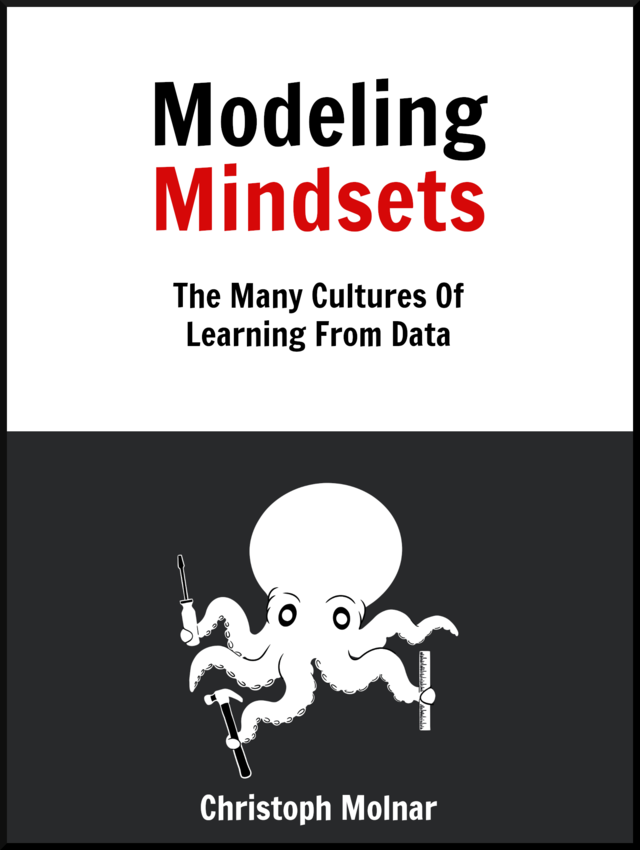
\includegraphics[width=0.5\textwidth]{figures/cover.png}
\end{minipage}
\end{frame}

\begin{frame}{Who is this guy?}
\begin{minipage}{0.5\textwidth}
  \begin{itemize}
    \item Interpretable Machine Learning-A Guide for Making Black Box Model Explainable
  \end{itemize}
\end{minipage}%
\begin{minipage}{0.5\textwidth}
  \centering
  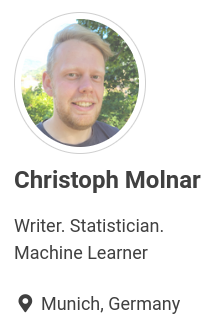
\includegraphics[width=0.5\textwidth]{figures/molnar.png}
\end{minipage}
\end{frame}

\begin{frame}{Modelling Mindsets}
  \color{Pink} Do not read if you dig on to the mindset you already know and are not open the other mindsets?! \color{Black}
  \begin{itemize}
    \item <1> Simple explanations with no math almost! 
    \item <2> Some interesting claims!
    \item <3> Funny anecdotes!
  \end{itemize}
\end{frame}

\begin{frame}{Big Battle}
    \centering
  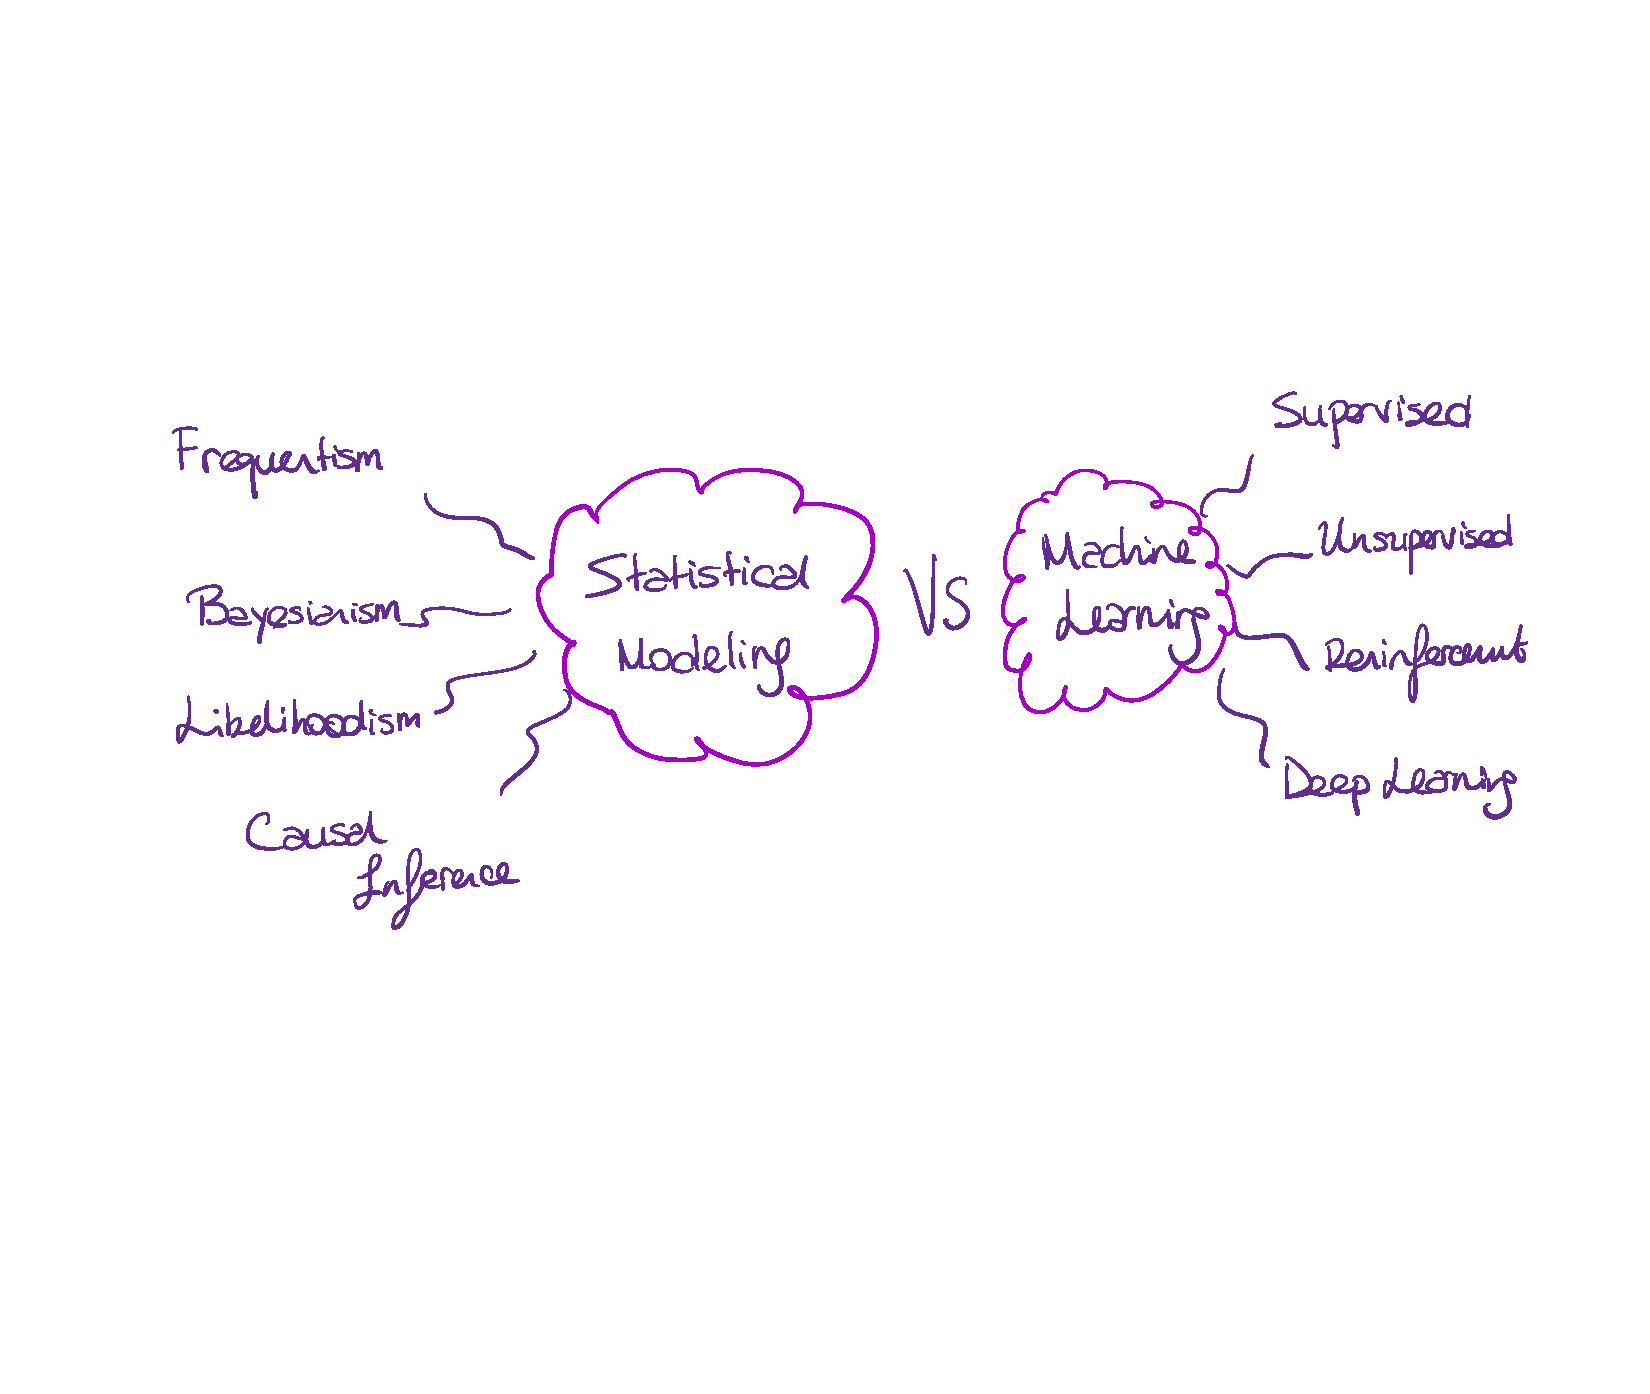
\includegraphics[scale=0.3]{figures/compare.pdf}
\end{frame}

\begin{frame}{Statistical Modeling vs Machine Learning}
  \textit{A machine learner walks along the beach. He sees a bottle in the sand opens it, and finds a genie who grants him a wish."I want to understand all machine leanring algorithms,"he says. The genie nods."Your wish is granted." The machine learner dissappears in a puff of smoke. In his place is a statistician.}
  \begin{itemize}
    \item Statistician starts analysis with a statistical hypothesis, interprets parameters, and so on. Even if the machine learner ends up with exactly the same model the interpretation and use in practice would be different!
    \item ML focuses on task performance.
  \end{itemize}
\end{frame}

\begin{frame}{The T-shaped Modeler}
  \begin{itemize}
    \item Pragmatic modeling requires many mindsets
    \item Don't try to be an expert on all mindsets...
    \item Become a T-shaped modeller!!!
  \end{itemize}
\end{frame}

\begin{frame}{Questions for you!}
  \begin{itemize}
    \item What is your mindset or are you already a T-shaped modeller?
    \item Modeller or Researcher?
  \end{itemize}
\end{frame}

\begin{frame}{}
  \color{Pink} Become an octopus! 
\end{frame}

\begin{frame}{Premises-Statistical Modeling}
  \begin{itemize}
    \item Frequintism: The world is best approached through probability distributions with fixed but unknown parameters!
    \item Bayesianism: The world is best approached through probability distributions with fixed but unknown parameters! 
    \item Likelihoodism: The world is best approached through probability distributions and likelihoods!
    \item Causal Inference: The world is best approached through causal reasoning!
  \end{itemize}
\end{frame}

\begin{frame}{Premises-Machine Learning}
  \begin{itemize}
    \item Supervised: The world is best approached by making predictions.
    \item Unsupervised: The world is best approached through identifying patterns.
    \item Reinforcement: The world is best approached through interacting with it.
    \item Deep: The world is best approached through deep neural networks.
  \end{itemize}
\end{frame}
\end{document}
